\begin{tikzpicture}
\def\figsize{0.9}
\node[anchor=south west] at (0, 0) {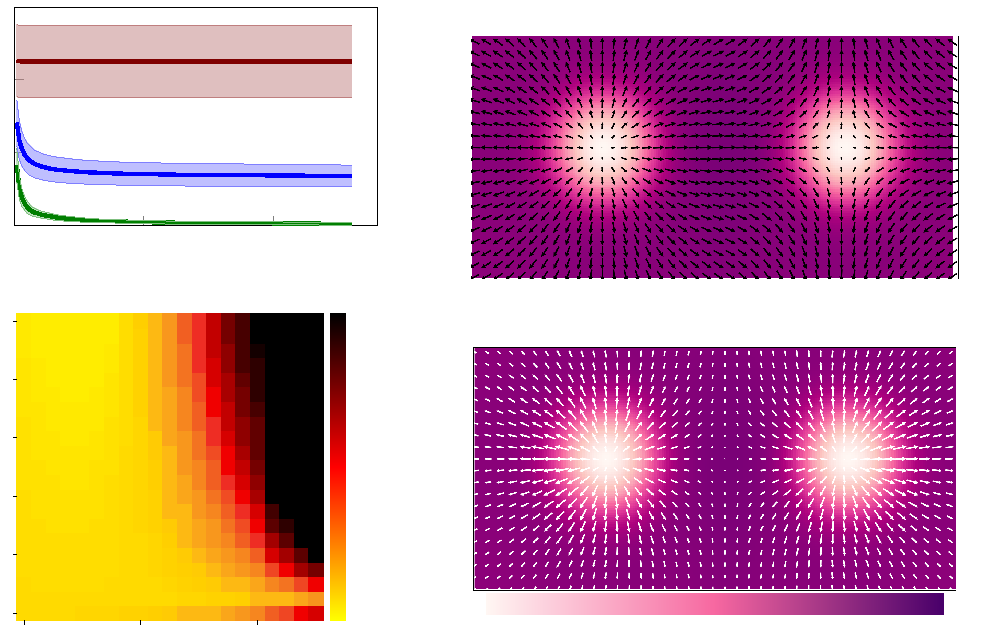
\includegraphics[width=0.9\linewidth]{Fig_twodefects_v4.pdf}};

% Panel (a)
%% Label
\node[anchor=south] at (-0.065*\figsize*\linewidth,0.62*\figsize*\linewidth) {(a)};
\node[rotate=90] at (-0.065*\figsize*\linewidth, 0.53*\figsize*\linewidth) {\# defects};
\node[align=center] at (0.2*\figsize*\linewidth, 0.37*\figsize*\linewidth) {Time $t$};
%% y-ticks
\def\spac{0.073*\figsize*\linewidth}
\def\offy{0.435*\figsize*\linewidth}
\foreach \ndef [count = \k] in {0, 100, 200}{%
    \pgfmathtruncatemacro{\posy}{ ((\k-1)*\spac+\offy}
    \node at (-0.01*\figsize*\linewidth, \posy pt) {\ndef}; 
}
%% x-ticks
\def\offx{0.04*\figsize*\linewidth}
\def\spac{0.13*\figsize*\linewidth}
\foreach \i [count = \n] in {0, $5\ex{5}$, $10^6$} {%
    \pgfmathtruncatemacro{\posx}{(\n-1)*\spac+\offx}
    \node at (\posx pt, 0.405*\figsize*\linewidth) {\i};
    % \draw (\posx,\posy) -- ++(0,-0.5);
}
%% Legend
\def\hh{0.675*\figsize*\linewidth}
\def\spac{0.105*\figsize*\linewidth}
\def\offx{0.06*\figsize*\linewidth}
\node at (\offx, \hh) {$\tau : $};
\filldraw[color=Maroon] (2*\offx,\hh) circle (0.075);
\node at (2*\offx,\hh)[right] {$0.2$};
\filldraw[color=blue] (2*\offx+\spac,\hh) circle (0.075);
\node at (2*\offx+\spac,\hh)[right] {$1.0$};
\filldraw[color=ao] (2*\offx+2*\spac,\hh) circle (0.075);
\node at (2*\offx+2*\spac,\hh)[right] {$10$};


% Panels (b) and (d)
\node[anchor=south west] at (0.47*\figsize*\linewidth,0.62*\figsize*\linewidth) {(b) Polarity};
\node[anchor=south west] at (0.47*\figsize*\linewidth,0.3*\figsize*\linewidth) {(d) Velocity};
\node at (0.51*\figsize*\linewidth, 0.0*\figsize*\linewidth){$0.58$};
\node at (0.75*\figsize*\linewidth, 0.0*\figsize*\linewidth){Density $\rho$};
\node at (0.95*\figsize*\linewidth, 0.0*\figsize*\linewidth){$0.6$};
\draw[white, thick] (0.502*\figsize*\linewidth, 0.38*\figsize*\linewidth) -- (0.742*\figsize*\linewidth, 0.38*\figsize*\linewidth) node[midway,above]{$1$};
\draw[white, thick] (0.502*\figsize*\linewidth, 0.063*\figsize*\linewidth) -- (0.742*\figsize*\linewidth, 0.063*\figsize*\linewidth) node[midway,above]{$1$};


% Panel (c)
%% Label
\node[anchor=south] at (-0.065*\figsize*\linewidth,0.3*\figsize*\linewidth) {(c)};
\node[rotate=90, align=center] at (-0.065*\figsize*\linewidth, 0.18*\figsize*\linewidth) {Activity $\zeta_\rho$};
\node[align=center] at (0.2*\figsize*\linewidth, -10pt) {Density $\rho_0$};
\node[align=center, rotate=90] at (0.445*\figsize*\linewidth, 0.17*\figsize*\linewidth) {Critical distance};
%% yticks (activity)
\def\spac{0.061*\figsize*\linewidth}
\def\offy{0.03*\figsize*\linewidth}
\foreach \zzr [count = \k] in {0,4,8,12,16,20}{%
    \pgfmathtruncatemacro{\posy}{ ((\k-1)*\spac+\offy}
    \node at (0.0*\figsize*\linewidth, \posy pt) {\zzr}; 
}
%% xticks (density)
\def\offx{0.04*\figsize*\linewidth}
\def\spac{0.12*\figsize*\linewidth}
\foreach \i [count = \n] in {0.4, 0.8, 1.2} {%
    \pgfmathtruncatemacro{\posx}{(\n-1)*\spac+\offx}
    \node at (\posx pt, 0pt) {\i};
    % \draw (\posx,\posy) -- ++(0,-0.5);
}
%% Colorbar ticks (critical distance)
\def\spac{0.074*\figsize*\linewidth}
\def\offy{0.03*\figsize*\linewidth}
\foreach \crd [count = \k] in {0.01, 0.5, 1, 1.5, 2}{%
    \pgfmathtruncatemacro{\posy}{ ((\k-1)*\spac+\offy}
    \ifnum \k = 1
        \node at (0.4*\figsize*\linewidth, 1pt) {\crd}; 
    \else
        \node at (0.4*\figsize*\linewidth, \posy pt) {\crd}; 
    \fi
}
\end{tikzpicture}